% Owner: Hassan Ashraf 24L-3073
\section{System Architecture and Contributions}
\label{sec:contributions}

\subsection{System Architecture}

Figure~\ref{fig:system} shows how the parts of ProcurePulse fit together. The
Deliverable~1 pipeline turns the raw downloads into chronological feature
files. Two independent model families read these files: the scikit-learn
models (Section~\ref{sec:classical}) and the LSTM (Section~\ref{sec:deep}).
Both write their predictions in one agreed format,
\texttt{results/predictions/<model>.csv}, which is the only connection between
the two halves of the code. The evaluation (Section~\ref{sec:evaluation}) and
the error analysis (Section~\ref{sec:error-bias}) read every prediction file,
so a new model only has to produce this file to be included. The whole system
runs with one command, \texttt{python main.py}, in eleven steps.

\begin{figure}[H]
  \centering
  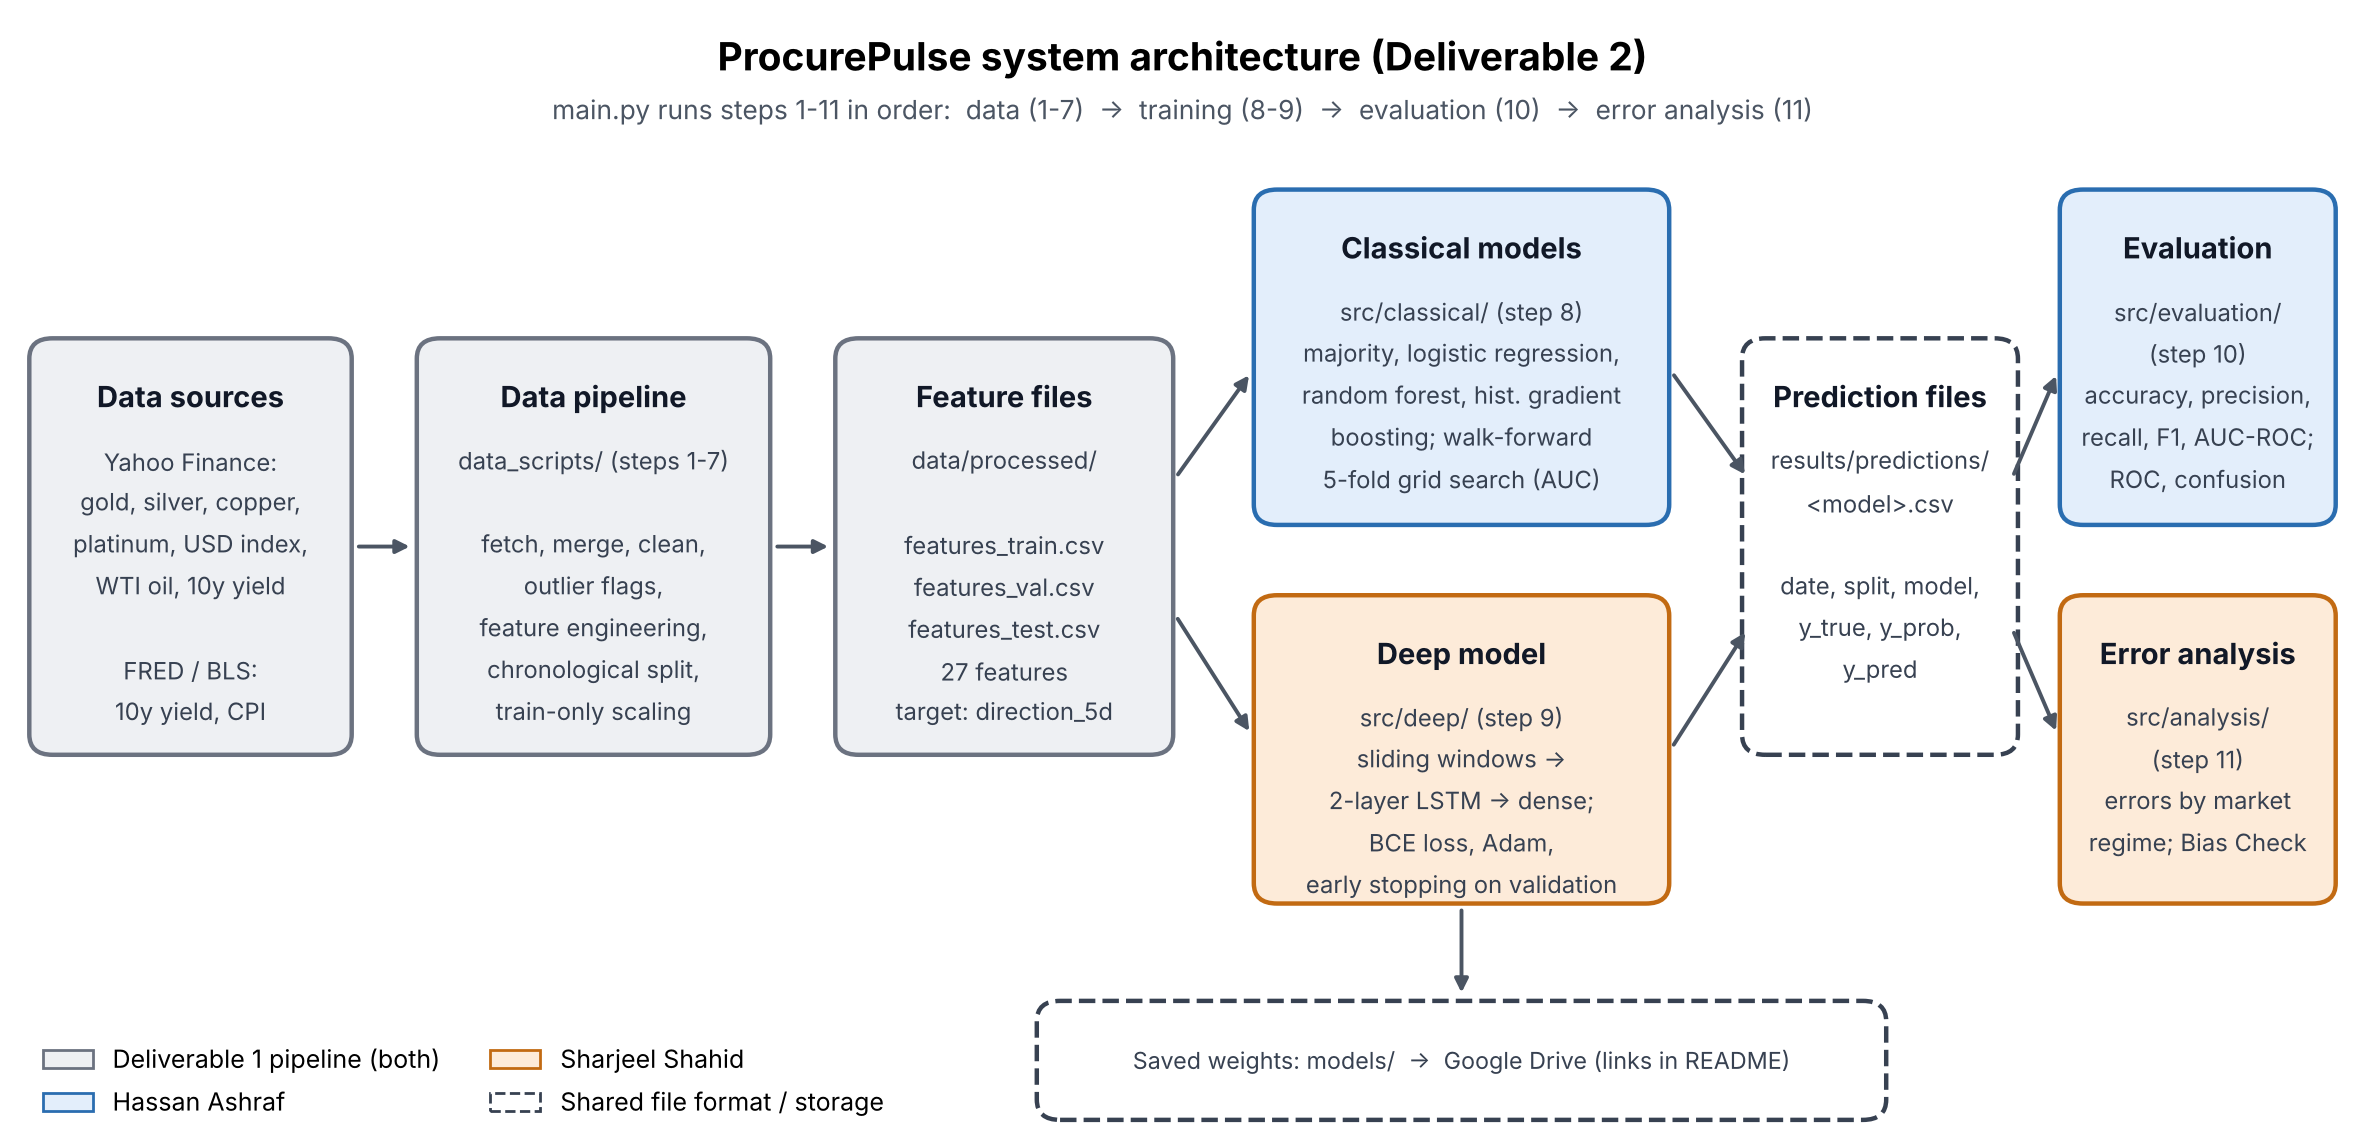
\includegraphics[width=\textwidth]{architecture/system_pipeline.png}
  \caption{System architecture. Colours show who built each part in Deliverable~2.}
  \label{fig:system}
\end{figure}

\subsection{Contribution Table}

Table~\ref{tab:contributions} lists every Deliverable~2 module, its files, the
Git author and the number of commits. The numbers are taken from the Git
history of the \texttt{main} branch (\texttt{git log --no-merges}); every module
was developed on its own feature branch and merged through a reviewed pull
request.

\begin{table}[H]
  \centering
  \small
  \sloppy
  \begin{tabular}{p{0.8cm}p{3.4cm}p{6.0cm}p{2.5cm}c}
    \toprule
    Task & Module & Files & Author & Commits \\
    \midrule
    A1 & Shared setup & \texttt{requirements.txt}, \texttt{.gitignore}, \texttt{report/main.tex} & Hassan Ashraf & 1 \\
    A2 & Classical data and models & \texttt{src/classical/data.py}, \texttt{models.py}, \texttt{tests/test\_classical.py} & Hassan Ashraf & 3 \\
    A3 & Classical training and tuning & \texttt{src/classical/train\_classical.py}, classical predictions, tuning table, feature importance & Hassan Ashraf & 3 \\
    A4 & Evaluation & \texttt{src/evaluation/}, \texttt{tests/test\_evaluation.py}, metrics, comparison table, charts & Hassan Ashraf & 6 \\
    A5 & Pipeline integration & \texttt{main.py} (steps 8--11) & Hassan Ashraf & 2 \\
    A6 & Report: classical models, evaluation, conclusion & Sections 7, 9 and conclusion, \texttt{refs\_a.bib} & Hassan Ashraf & 3 \\
    A7 & Architecture and contributions & \texttt{11\_contributions.tex}, system diagram & Hassan Ashraf & 1 \\
    \midrule
    % Sharjeel's rows: fill in from the Git history once B1-B7 are merged.
    B1--B3 & LSTM dataset, model and training & \texttt{src/deep/} & Sharjeel Shahid & -- \\
    B4 & LSTM tuning and training curves & \texttt{src/deep/tune\_lstm.py}, \texttt{plot\_training.py} & Sharjeel Shahid & -- \\
    B5 & Error analysis and bias check & \texttt{src/analysis/} & Sharjeel Shahid & -- \\
    B6 & Report: deep model, error analysis & Sections on the LSTM and the Bias Check, \texttt{refs\_b.bib} & Sharjeel Shahid & -- \\
    B7 & README and weights links & \texttt{README.md} & Sharjeel Shahid & -- \\
    \bottomrule
  \end{tabular}
  \caption{Contribution Table for Deliverable~2 (from the Git history of \texttt{main}).}
  \label{tab:contributions}
\end{table}